% Options for packages loaded elsewhere
\PassOptionsToPackage{unicode}{hyperref}
\PassOptionsToPackage{hyphens}{url}
\PassOptionsToPackage{dvipsnames,svgnames,x11names}{xcolor}
%
\documentclass[
  ignorenonframetext,
]{beamer}
\usepackage{pgfpages}
\setbeamertemplate{caption}[numbered]
\setbeamertemplate{caption label separator}{: }
\setbeamercolor{caption name}{fg=normal text.fg}
\beamertemplatenavigationsymbolsempty
% Prevent slide breaks in the middle of a paragraph
\widowpenalties 1 10000
\raggedbottom
\setbeamertemplate{part page}{
  \centering
  \begin{beamercolorbox}[sep=16pt,center]{part title}
    \usebeamerfont{part title}\insertpart\par
  \end{beamercolorbox}
}
\setbeamertemplate{section page}{
  \centering
  \begin{beamercolorbox}[sep=12pt,center]{part title}
    \usebeamerfont{section title}\insertsection\par
  \end{beamercolorbox}
}
\setbeamertemplate{subsection page}{
  \centering
  \begin{beamercolorbox}[sep=8pt,center]{part title}
    \usebeamerfont{subsection title}\insertsubsection\par
  \end{beamercolorbox}
}
\AtBeginPart{
  \frame{\partpage}
}
\AtBeginSection{
  \ifbibliography
  \else
    \frame{\sectionpage}
  \fi
}
\AtBeginSubsection{
  \frame{\subsectionpage}
}
\usepackage{amsmath,amssymb}
\usepackage{lmodern}
\usepackage{iftex}
\ifPDFTeX
  \usepackage[T1]{fontenc}
  \usepackage[utf8]{inputenc}
  \usepackage{textcomp} % provide euro and other symbols
\else % if luatex or xetex
  \usepackage{unicode-math}
  \defaultfontfeatures{Scale=MatchLowercase}
  \defaultfontfeatures[\rmfamily]{Ligatures=TeX,Scale=1}
\fi
% Use upquote if available, for straight quotes in verbatim environments
\IfFileExists{upquote.sty}{\usepackage{upquote}}{}
\IfFileExists{microtype.sty}{% use microtype if available
  \usepackage[]{microtype}
  \UseMicrotypeSet[protrusion]{basicmath} % disable protrusion for tt fonts
}{}
\makeatletter
\@ifundefined{KOMAClassName}{% if non-KOMA class
  \IfFileExists{parskip.sty}{%
    \usepackage{parskip}
  }{% else
    \setlength{\parindent}{0pt}
    \setlength{\parskip}{6pt plus 2pt minus 1pt}}
}{% if KOMA class
  \KOMAoptions{parskip=half}}
\makeatother
\usepackage{xcolor}
\newif\ifbibliography
\usepackage{color}
\usepackage{fancyvrb}
\newcommand{\VerbBar}{|}
\newcommand{\VERB}{\Verb[commandchars=\\\{\}]}
\DefineVerbatimEnvironment{Highlighting}{Verbatim}{commandchars=\\\{\}}
% Add ',fontsize=\small' for more characters per line
\usepackage{framed}
\definecolor{shadecolor}{RGB}{248,248,248}
\newenvironment{Shaded}{\begin{snugshade}}{\end{snugshade}}
\newcommand{\AlertTok}[1]{\textcolor[rgb]{0.94,0.16,0.16}{#1}}
\newcommand{\AnnotationTok}[1]{\textcolor[rgb]{0.56,0.35,0.01}{\textbf{\textit{#1}}}}
\newcommand{\AttributeTok}[1]{\textcolor[rgb]{0.77,0.63,0.00}{#1}}
\newcommand{\BaseNTok}[1]{\textcolor[rgb]{0.00,0.00,0.81}{#1}}
\newcommand{\BuiltInTok}[1]{#1}
\newcommand{\CharTok}[1]{\textcolor[rgb]{0.31,0.60,0.02}{#1}}
\newcommand{\CommentTok}[1]{\textcolor[rgb]{0.56,0.35,0.01}{\textit{#1}}}
\newcommand{\CommentVarTok}[1]{\textcolor[rgb]{0.56,0.35,0.01}{\textbf{\textit{#1}}}}
\newcommand{\ConstantTok}[1]{\textcolor[rgb]{0.00,0.00,0.00}{#1}}
\newcommand{\ControlFlowTok}[1]{\textcolor[rgb]{0.13,0.29,0.53}{\textbf{#1}}}
\newcommand{\DataTypeTok}[1]{\textcolor[rgb]{0.13,0.29,0.53}{#1}}
\newcommand{\DecValTok}[1]{\textcolor[rgb]{0.00,0.00,0.81}{#1}}
\newcommand{\DocumentationTok}[1]{\textcolor[rgb]{0.56,0.35,0.01}{\textbf{\textit{#1}}}}
\newcommand{\ErrorTok}[1]{\textcolor[rgb]{0.64,0.00,0.00}{\textbf{#1}}}
\newcommand{\ExtensionTok}[1]{#1}
\newcommand{\FloatTok}[1]{\textcolor[rgb]{0.00,0.00,0.81}{#1}}
\newcommand{\FunctionTok}[1]{\textcolor[rgb]{0.00,0.00,0.00}{#1}}
\newcommand{\ImportTok}[1]{#1}
\newcommand{\InformationTok}[1]{\textcolor[rgb]{0.56,0.35,0.01}{\textbf{\textit{#1}}}}
\newcommand{\KeywordTok}[1]{\textcolor[rgb]{0.13,0.29,0.53}{\textbf{#1}}}
\newcommand{\NormalTok}[1]{#1}
\newcommand{\OperatorTok}[1]{\textcolor[rgb]{0.81,0.36,0.00}{\textbf{#1}}}
\newcommand{\OtherTok}[1]{\textcolor[rgb]{0.56,0.35,0.01}{#1}}
\newcommand{\PreprocessorTok}[1]{\textcolor[rgb]{0.56,0.35,0.01}{\textit{#1}}}
\newcommand{\RegionMarkerTok}[1]{#1}
\newcommand{\SpecialCharTok}[1]{\textcolor[rgb]{0.00,0.00,0.00}{#1}}
\newcommand{\SpecialStringTok}[1]{\textcolor[rgb]{0.31,0.60,0.02}{#1}}
\newcommand{\StringTok}[1]{\textcolor[rgb]{0.31,0.60,0.02}{#1}}
\newcommand{\VariableTok}[1]{\textcolor[rgb]{0.00,0.00,0.00}{#1}}
\newcommand{\VerbatimStringTok}[1]{\textcolor[rgb]{0.31,0.60,0.02}{#1}}
\newcommand{\WarningTok}[1]{\textcolor[rgb]{0.56,0.35,0.01}{\textbf{\textit{#1}}}}
\usepackage{graphicx}
\makeatletter
\def\maxwidth{\ifdim\Gin@nat@width>\linewidth\linewidth\else\Gin@nat@width\fi}
\def\maxheight{\ifdim\Gin@nat@height>\textheight\textheight\else\Gin@nat@height\fi}
\makeatother
% Scale images if necessary, so that they will not overflow the page
% margins by default, and it is still possible to overwrite the defaults
% using explicit options in \includegraphics[width, height, ...]{}
\setkeys{Gin}{width=\maxwidth,height=\maxheight,keepaspectratio}
% Set default figure placement to htbp
\makeatletter
\def\fps@figure{htbp}
\makeatother
\setlength{\emergencystretch}{3em} % prevent overfull lines
\providecommand{\tightlist}{%
  \setlength{\itemsep}{0pt}\setlength{\parskip}{0pt}}
\setcounter{secnumdepth}{-\maxdimen} % remove section numbering
\usepackage{graphicx}
\usepackage{bm}
\usepackage{array}
\usepackage{amsmath}
\usepackage{amsthm}
\usepackage{amsfonts}
\usepackage{amssymb}
\usepackage{tikz-cd}
\usepackage{url}
\definecolor{foreground}{RGB}{255,255,255}
\definecolor{background}{RGB}{34,28,54}
\definecolor{title}{RGB}{105,165,255}
\definecolor{gray}{RGB}{175,175,175}
\definecolor{lightgray}{RGB}{225,225,225}
\definecolor{subtitle}{RGB}{232,234,255}
\definecolor{hilight}{RGB}{112,224,255}
\definecolor{vhilight}{RGB}{255,111,207}
\setbeamertemplate{footline}[page number]
\ifLuaTeX
  \usepackage{selnolig}  % disable illegal ligatures
\fi
\IfFileExists{bookmark.sty}{\usepackage{bookmark}}{\usepackage{hyperref}}
\IfFileExists{xurl.sty}{\usepackage{xurl}}{} % add URL line breaks if available
\urlstyle{same} % disable monospaced font for URLs
\hypersetup{
  pdftitle={STAT 528 - Advanced Regression Analysis II},
  pdfauthor={Count response regression (part II)},
  colorlinks=true,
  linkcolor={Maroon},
  filecolor={Maroon},
  citecolor={Blue},
  urlcolor={blue},
  pdfcreator={LaTeX via pandoc}}

\title{STAT 528 - Advanced Regression Analysis II}
\author{Count response regression (part II)}
\date{}
\institute{Daniel J. Eck\\
Department of Statistics\\
University of Illinois}

\begin{document}
\frame{\titlepage}

\begin{frame}
\newcommand{\R}{\mathbb{R}}
\newcommand{\Prob}{\mathbb{P}}
\newcommand{\Proj}{\textbf{P}}
\newcommand{\Hcal}{\mathcal{H}}
\newcommand{\rootn}{\sqrt{n}}
\newcommand{\p}{\mathbf{p}}
\newcommand{\E}{\text{E}}
\newcommand{\Var}{\text{Var}}
\newcommand{\Cov}{\text{Cov}}
\newcommand{\mubf}{\bm{\mu}}
\newcommand{\logit}{\text{logit}}

\newtheorem{cor}{Corollary}
\newtheorem{lem}{Lemma}
\newtheorem{thm}{Theorem}
\newtheorem{defn}{Definition}
\newtheorem{prop}{Proposition}
\end{frame}

\begin{frame}{Last time}
\protect\hypertarget{last-time}{}
\begin{itemize}
\tightlist
\item
  Poisson regression
\item
  Residual diagnostics
\item
  Data analysis
\end{itemize}
\end{frame}

\begin{frame}{Learning Objectives Today}
\protect\hypertarget{learning-objectives-today}{}
\begin{itemize}
\tightlist
\item
  Overdispersion
\item
  gala data analysis
\item
  Negative Binomial regression
\item
  Zero Inflated Count Models
\end{itemize}
\end{frame}

\begin{frame}{}
\protect\hypertarget{section}{}
When the mechanism is not known, we can introduce a dispersion parameter
\(\phi\) such that \(\mathrm{Var}(Y) = \phi \mathrm{E}(Y) = \phi\mu\).
This decouples the variance from the mean.

\vspace{12pt}

The case \(\phi = 1\) is the regular Poisson regression case, while
\(\phi > 1\) is overdispersion and \(\phi < 1\) is underdispersion.

\vspace{12pt}

A common explanation for large deviance (or poor fit) is the presence of
a few outliers.

\vspace{12pt}

When large number of points are identified as outliers, they become
unexceptional, and it may be the case that the error distribution is
misspecified.
\end{frame}

\begin{frame}{}
\protect\hypertarget{section-1}{}
In the presence of overdispersion, the exponential family takes on a
different functional form \begin{equation} \label{expofamdisp}
  f(y|\theta,\phi) = \exp\left(\frac{\langle y,\theta\rangle- c(\theta)}{a(\phi)} - b(y,\phi) \right),
\end{equation} where

\begin{itemize}
\tightlist
\item
  \(y\), \(\theta\), and \(c(\theta)\) are as before
\item
  \(\phi\) is a dispersion parameter
\item
  \(b(y,\phi)\) is a function of the data \(y\) and the dispersion
  parameter \(\phi\).
\end{itemize}

\vspace{12pt}

Notice that the density \eqref{expofamdisp} is a generalization of the
exponential family density which specifies that \(a(\phi) = 1\) and
\(b(y,\phi) = \log(h(y))\).

\vspace{12pt}

This is not a canonical exponential family model. What happens to
sufficiency?
\end{frame}

\begin{frame}{}
\protect\hypertarget{section-2}{}
Note that the dispersion parameter can be estimated using \[
  \hat{\phi} = \frac{\sum_{i=1}^n(y - \hat\mu_i)^2/\hat\mu_i}{n-p}.
\] Notice that the estimation of the dispersion and the regression
parameters is independent, so choosing a dispersion other than one has
no effect on the regression parameter estimates.
\end{frame}

\begin{frame}[fragile]{}
\protect\hypertarget{section-3}{}
We investigate the overdispersed Poisson regression model with respect
to the Galapogas data.

\vspace{12pt}

\begin{Shaded}
\begin{Highlighting}[]
\NormalTok{n }\OtherTok{\textless{}{-}} \FunctionTok{nrow}\NormalTok{(gala)}
\NormalTok{p }\OtherTok{\textless{}{-}} \FunctionTok{length}\NormalTok{(}\FunctionTok{coef}\NormalTok{(m1))}
\NormalTok{y }\OtherTok{\textless{}{-}}\NormalTok{ gala}\SpecialCharTok{$}\NormalTok{Species}

\DocumentationTok{\#\# estimate dispersion directly}
\NormalTok{fits }\OtherTok{\textless{}{-}} \FunctionTok{predict}\NormalTok{(m1, }\AttributeTok{type =} \StringTok{"response"}\NormalTok{)}
\NormalTok{dp }\OtherTok{\textless{}{-}} \FunctionTok{sum}\NormalTok{((y }\SpecialCharTok{{-}}\NormalTok{ fits)}\SpecialCharTok{\^{}}\DecValTok{2}\SpecialCharTok{/}\NormalTok{fits) }\SpecialCharTok{/}\NormalTok{ (n }\SpecialCharTok{{-}}\NormalTok{ p)}
\NormalTok{dp}
\end{Highlighting}
\end{Shaded}

\begin{verbatim}
## [1] 29.9553
\end{verbatim}
\end{frame}

\begin{frame}[fragile]{}
\protect\hypertarget{section-4}{}
\tiny

\begin{Shaded}
\begin{Highlighting}[]
\FunctionTok{summary}\NormalTok{(m1, }\AttributeTok{dispersion =}\NormalTok{ dp)}
\end{Highlighting}
\end{Shaded}

\begin{verbatim}
## 
## Call:
## glm(formula = Species ~ Elevation + Nearest + Scruz + Adjacent + 
##     Size, family = "poisson", data = gala, x = TRUE)
## 
## Deviance Residuals: 
##      Min        1Q    Median        3Q       Max  
## -10.3723   -3.5214   -0.9947    1.7193   10.6627  
## 
## Coefficients:
##               Estimate Std. Error z value Pr(>|z|)    
## (Intercept)  2.7897965  0.4437393   6.287 3.24e-10 ***
## Elevation    0.0009361  0.0002957   3.166  0.00154 ** 
## Nearest      0.0064693  0.0095646   0.676  0.49880    
## Scruz       -0.0062665  0.0034307  -1.827  0.06776 .  
## Adjacent    -0.0002858  0.0001620  -1.764  0.07781 .  
## Size2        1.1276155  0.5218686   2.161  0.03072 *  
## Size3        2.0586771  0.5155262   3.993 6.51e-05 ***
## ---
## Signif. codes:  0 '***' 0.001 '**' 0.01 '*' 0.05 '.' 0.1 ' ' 1
## 
## (Dispersion parameter for poisson family taken to be 29.9553)
## 
##     Null deviance: 3510.73  on 29  degrees of freedom
## Residual deviance:  594.18  on 23  degrees of freedom
## AIC: 769.01
## 
## Number of Fisher Scoring iterations: 5
\end{verbatim}
\end{frame}

\begin{frame}[fragile]{}
\protect\hypertarget{section-5}{}
\tiny

\begin{Shaded}
\begin{Highlighting}[]
\NormalTok{m2 }\OtherTok{\textless{}{-}} \FunctionTok{glm}\NormalTok{(Species }\SpecialCharTok{\textasciitilde{}}\NormalTok{ Elevation }\SpecialCharTok{+}\NormalTok{ Nearest }\SpecialCharTok{+}\NormalTok{ Scruz }\SpecialCharTok{+}\NormalTok{ Adjacent }\SpecialCharTok{+}\NormalTok{ Size, }
          \AttributeTok{family =} \StringTok{"quasipoisson"}\NormalTok{, }\AttributeTok{data =}\NormalTok{ gala, }\AttributeTok{x =} \ConstantTok{TRUE}\NormalTok{)}
\FunctionTok{summary}\NormalTok{(m2)}
\end{Highlighting}
\end{Shaded}

\begin{verbatim}
## 
## Call:
## glm(formula = Species ~ Elevation + Nearest + Scruz + Adjacent + 
##     Size, family = "quasipoisson", data = gala, x = TRUE)
## 
## Deviance Residuals: 
##      Min        1Q    Median        3Q       Max  
## -10.3723   -3.5214   -0.9947    1.7193   10.6627  
## 
## Coefficients:
##               Estimate Std. Error t value Pr(>|t|)    
## (Intercept)  2.7897965  0.4437452   6.287 2.05e-06 ***
## Elevation    0.0009361  0.0002957   3.166 0.004314 ** 
## Nearest      0.0064693  0.0095648   0.676 0.505552    
## Scruz       -0.0062665  0.0034308  -1.827 0.080777 .  
## Adjacent    -0.0002858  0.0001621  -1.764 0.091094 .  
## Size2        1.1276155  0.5218755   2.161 0.041376 *  
## Size3        2.0586771  0.5155330   3.993 0.000572 ***
## ---
## Signif. codes:  0 '***' 0.001 '**' 0.01 '*' 0.05 '.' 0.1 ' ' 1
## 
## (Dispersion parameter for quasipoisson family taken to be 29.95609)
## 
##     Null deviance: 3510.73  on 29  degrees of freedom
## Residual deviance:  594.18  on 23  degrees of freedom
## AIC: NA
## 
## Number of Fisher Scoring iterations: 5
\end{verbatim}
\end{frame}

\begin{frame}[fragile]{}
\protect\hypertarget{section-6}{}
In this case the dispersion is quite large leading to an increase in
standard errors of over a factor of 5

\vspace{12pt}
\tiny

\begin{Shaded}
\begin{Highlighting}[]
\FunctionTok{c}\NormalTok{(dp, }\FunctionTok{sqrt}\NormalTok{(dp))}
\end{Highlighting}
\end{Shaded}

\begin{verbatim}
## [1] 29.955296  5.473143
\end{verbatim}

\begin{Shaded}
\begin{Highlighting}[]
\NormalTok{se }\OtherTok{\textless{}{-}} \ControlFlowTok{function}\NormalTok{(model) }\FunctionTok{sqrt}\NormalTok{(}\FunctionTok{diag}\NormalTok{(}\FunctionTok{vcov}\NormalTok{(model)))}
\FunctionTok{round}\NormalTok{(}\FunctionTok{data.frame}\NormalTok{(}\AttributeTok{coef.m1=}\FunctionTok{coef}\NormalTok{(m1), }\AttributeTok{coef.m2=}\FunctionTok{coef}\NormalTok{(m2), }\AttributeTok{se.m1=}\FunctionTok{se}\NormalTok{(m1), }\AttributeTok{se.m2=}\FunctionTok{se}\NormalTok{(m2), }
                 \AttributeTok{ratio=}\FunctionTok{se}\NormalTok{(m2)}\SpecialCharTok{/}\FunctionTok{se}\NormalTok{(m1)), }\DecValTok{4}\NormalTok{)}
\end{Highlighting}
\end{Shaded}

\begin{verbatim}
##             coef.m1 coef.m2  se.m1  se.m2  ratio
## (Intercept)  2.7898  2.7898 0.0811 0.4437 5.4732
## Elevation    0.0009  0.0009 0.0001 0.0003 5.4732
## Nearest      0.0065  0.0065 0.0017 0.0096 5.4732
## Scruz       -0.0063 -0.0063 0.0006 0.0034 5.4732
## Adjacent    -0.0003 -0.0003 0.0000 0.0002 5.4732
## Size2        1.1276  1.1276 0.0954 0.5219 5.4732
## Size3        2.0587  2.0587 0.0942 0.5155 5.4732
\end{verbatim}
\end{frame}

\begin{frame}{}
\protect\hypertarget{section-7}{}
The overdispersed Poisson model clearly offers improvements to the
residuals vs fitted values plot

\vspace{12pt}
\tiny

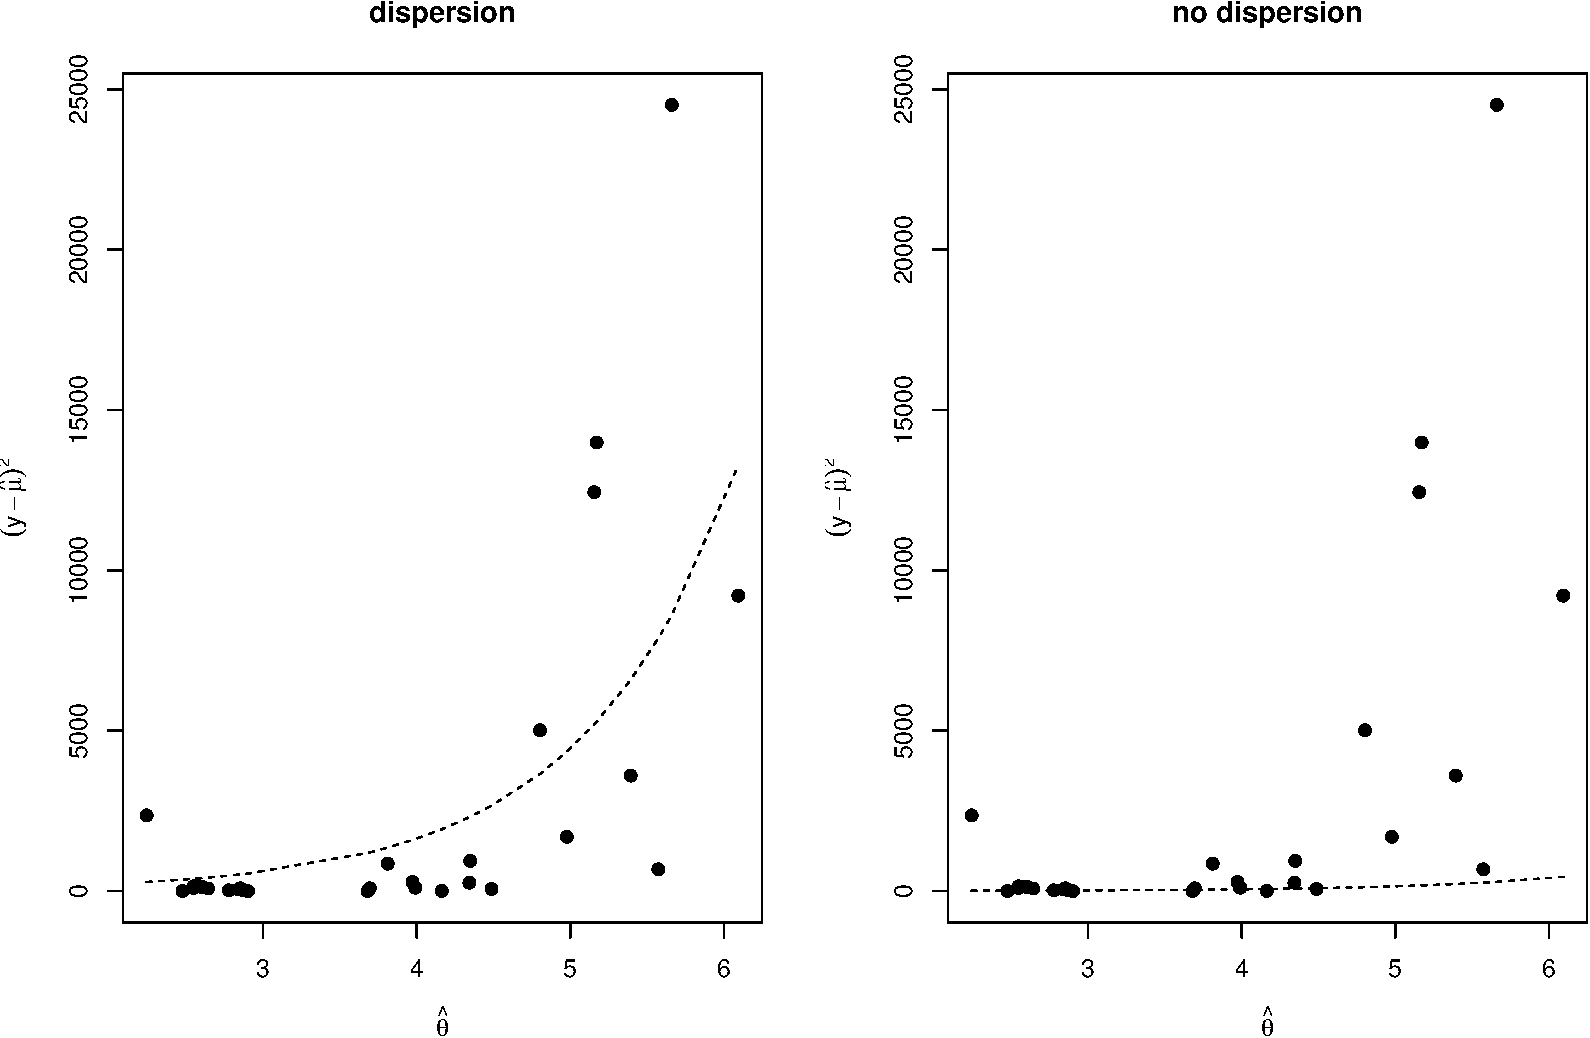
\includegraphics{week5_p1_files/figure-beamer/unnamed-chunk-6-1.pdf}
\end{frame}

\begin{frame}{}
\protect\hypertarget{section-8}{}
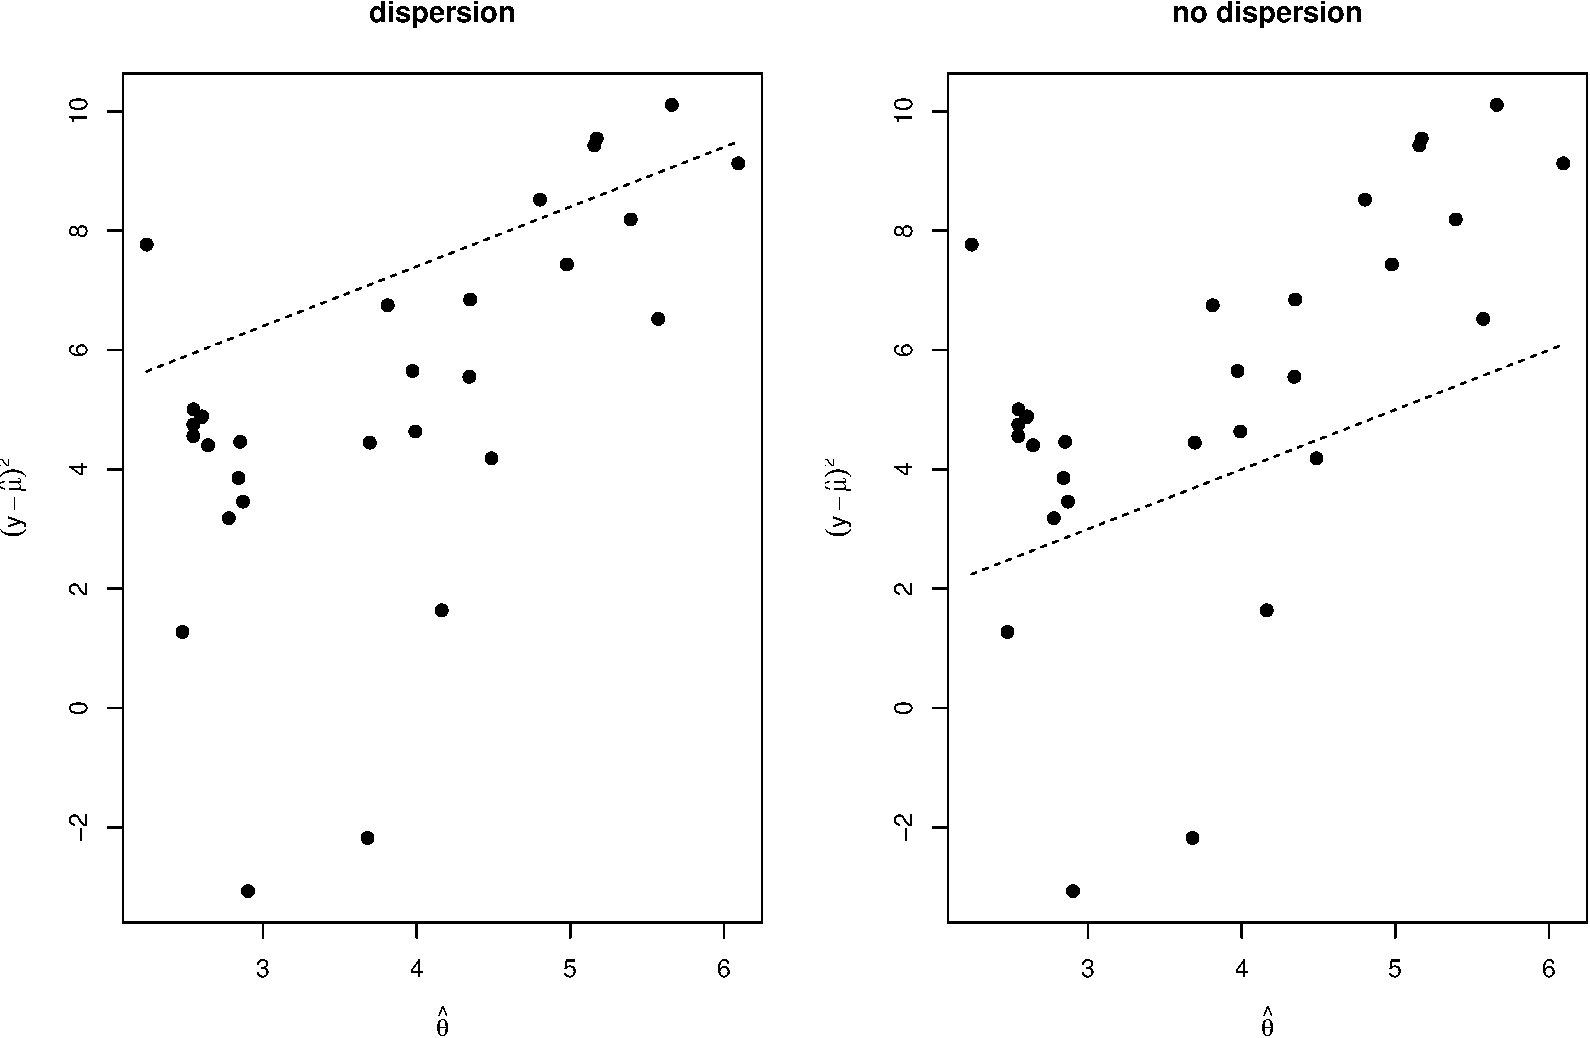
\includegraphics{week5_p1_files/figure-beamer/unnamed-chunk-7-1.pdf}
\end{frame}

\begin{frame}[fragile]{}
\protect\hypertarget{section-9}{}
The \texttt{AER} package includes a function that allows for one to
\href{https://www.sciencedirect.com/science/article/abs/pii/030440769090014K}{test
whether or not dispersion is present}. We can see that dispersion is
present at most reasonable significance testing levels.

\vspace{12pt}
\tiny

\begin{Shaded}
\begin{Highlighting}[]
\FunctionTok{library}\NormalTok{(AER)}
\FunctionTok{dispersiontest}\NormalTok{(m1, }\AttributeTok{trafo=}\DecValTok{1}\NormalTok{)}
\end{Highlighting}
\end{Shaded}

\begin{verbatim}
## 
##  Overdispersion test
## 
## data:  m1
## z = 2.5007, p-value = 0.006198
## alternative hypothesis: true alpha is greater than 0
## sample estimates:
##    alpha 
## 21.92009
\end{verbatim}

\vspace{12pt}
\normalsize

Note that the \texttt{AER} package defines dispersion differently than
the \texttt{glm} function.
\end{frame}

\begin{frame}[fragile]{}
\protect\hypertarget{section-10}{}
Let's consider our better performing model from last time.

\vspace{12pt}
\tiny

\begin{Shaded}
\begin{Highlighting}[]
\NormalTok{m3 }\OtherTok{\textless{}{-}} \FunctionTok{glm}\NormalTok{(Species }\SpecialCharTok{\textasciitilde{}}\NormalTok{ Elevation }\SpecialCharTok{+} \FunctionTok{I}\NormalTok{(Elevation}\SpecialCharTok{\^{}}\DecValTok{2}\NormalTok{) }\SpecialCharTok{+}\NormalTok{ Nearest }\SpecialCharTok{+}\NormalTok{ Scruz }\SpecialCharTok{+} 
            \FunctionTok{I}\NormalTok{(Scruz}\SpecialCharTok{\^{}}\DecValTok{2}\NormalTok{) }\SpecialCharTok{+}\NormalTok{ Adjacent }\SpecialCharTok{+} 
\NormalTok{            Area }\SpecialCharTok{+} \FunctionTok{I}\NormalTok{(Area}\SpecialCharTok{\^{}}\DecValTok{2}\NormalTok{), }\AttributeTok{family =} \StringTok{"poisson"}\NormalTok{, }\AttributeTok{data =}\NormalTok{ gala, }\AttributeTok{x =} \ConstantTok{TRUE}\NormalTok{)}
\end{Highlighting}
\end{Shaded}
\end{frame}

\begin{frame}[fragile]{}
\protect\hypertarget{section-11}{}
This model appears to also be over dispersed.

\vspace{12pt}
\tiny

\begin{Shaded}
\begin{Highlighting}[]
\NormalTok{p }\OtherTok{\textless{}{-}} \FunctionTok{length}\NormalTok{(}\FunctionTok{coef}\NormalTok{(m3))}

\NormalTok{fits }\OtherTok{\textless{}{-}} \FunctionTok{predict}\NormalTok{(m3, }\AttributeTok{type =} \StringTok{"response"}\NormalTok{)}
\NormalTok{dp3 }\OtherTok{\textless{}{-}} \FunctionTok{sum}\NormalTok{((y }\SpecialCharTok{{-}}\NormalTok{ fits)}\SpecialCharTok{\^{}}\DecValTok{2}\SpecialCharTok{/}\NormalTok{fits) }\SpecialCharTok{/}\NormalTok{ (n }\SpecialCharTok{{-}}\NormalTok{ p)}
\NormalTok{dp3}
\end{Highlighting}
\end{Shaded}

\begin{verbatim}
## [1] 17.84607
\end{verbatim}

\begin{Shaded}
\begin{Highlighting}[]
\FunctionTok{dispersiontest}\NormalTok{(m3, }\AttributeTok{trafo=}\DecValTok{1}\NormalTok{)}
\end{Highlighting}
\end{Shaded}

\begin{verbatim}
## 
##  Overdispersion test
## 
## data:  m3
## z = 4.2173, p-value = 1.236e-05
## alternative hypothesis: true alpha is greater than 0
## sample estimates:
##    alpha 
## 11.47278
\end{verbatim}
\end{frame}

\begin{frame}{}
\protect\hypertarget{section-12}{}
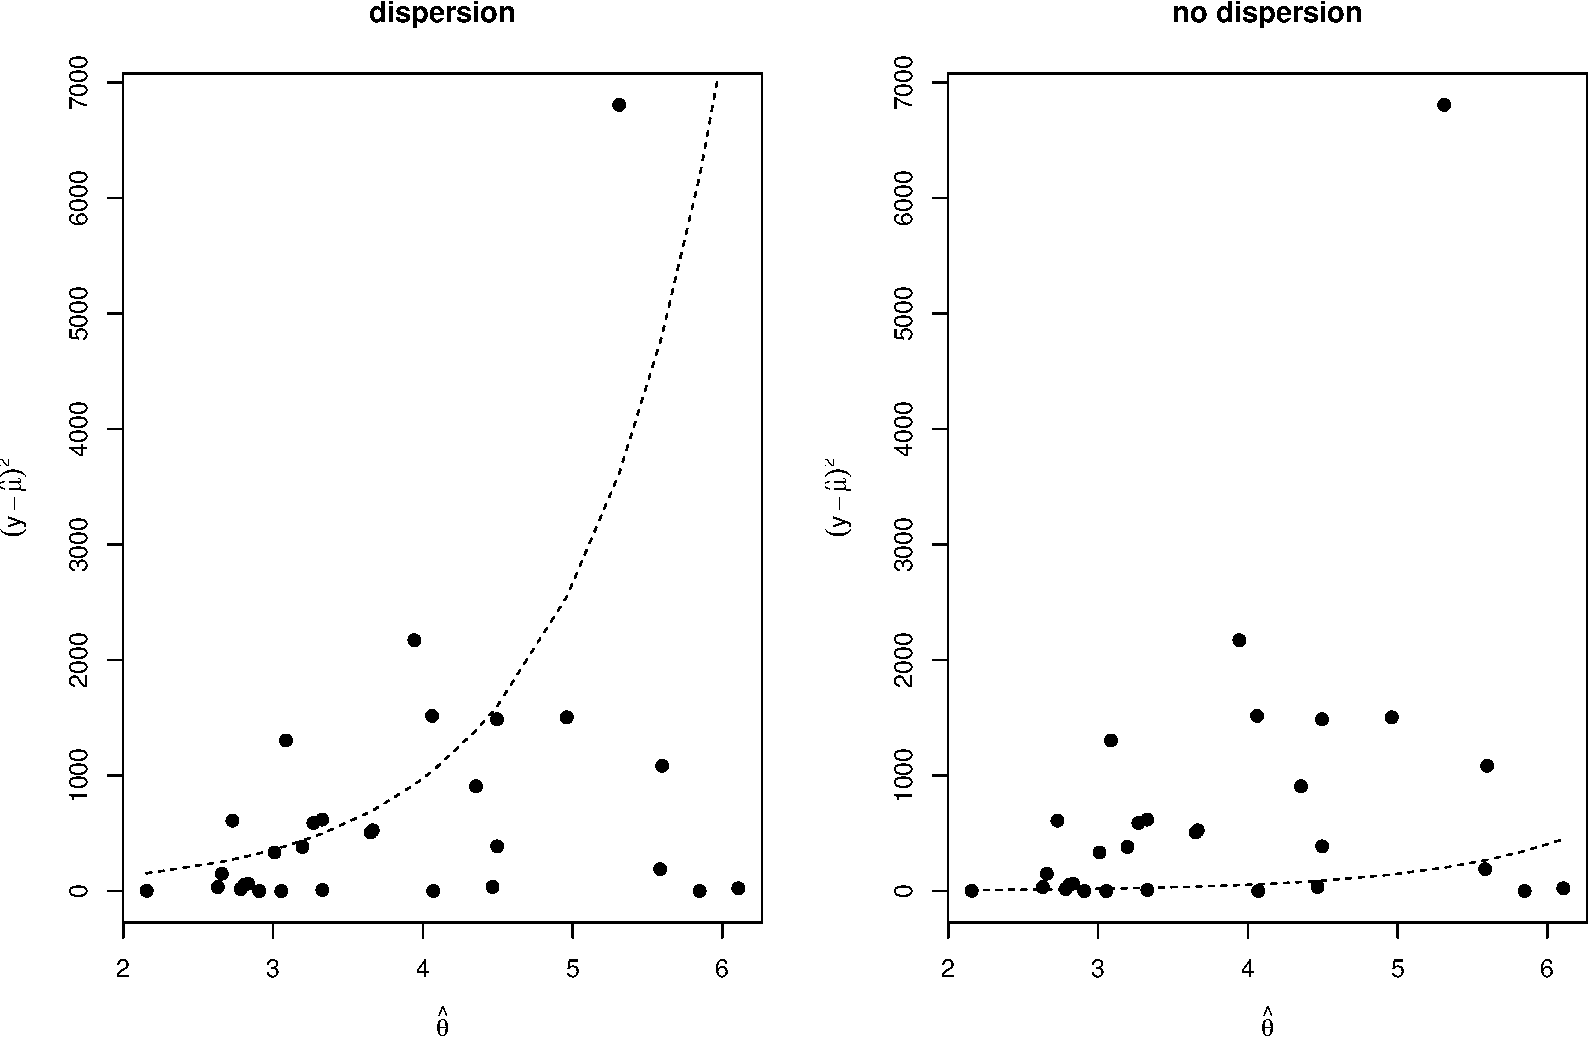
\includegraphics{week5_p1_files/figure-beamer/unnamed-chunk-11-1.pdf}
\end{frame}

\begin{frame}{}
\protect\hypertarget{section-13}{}
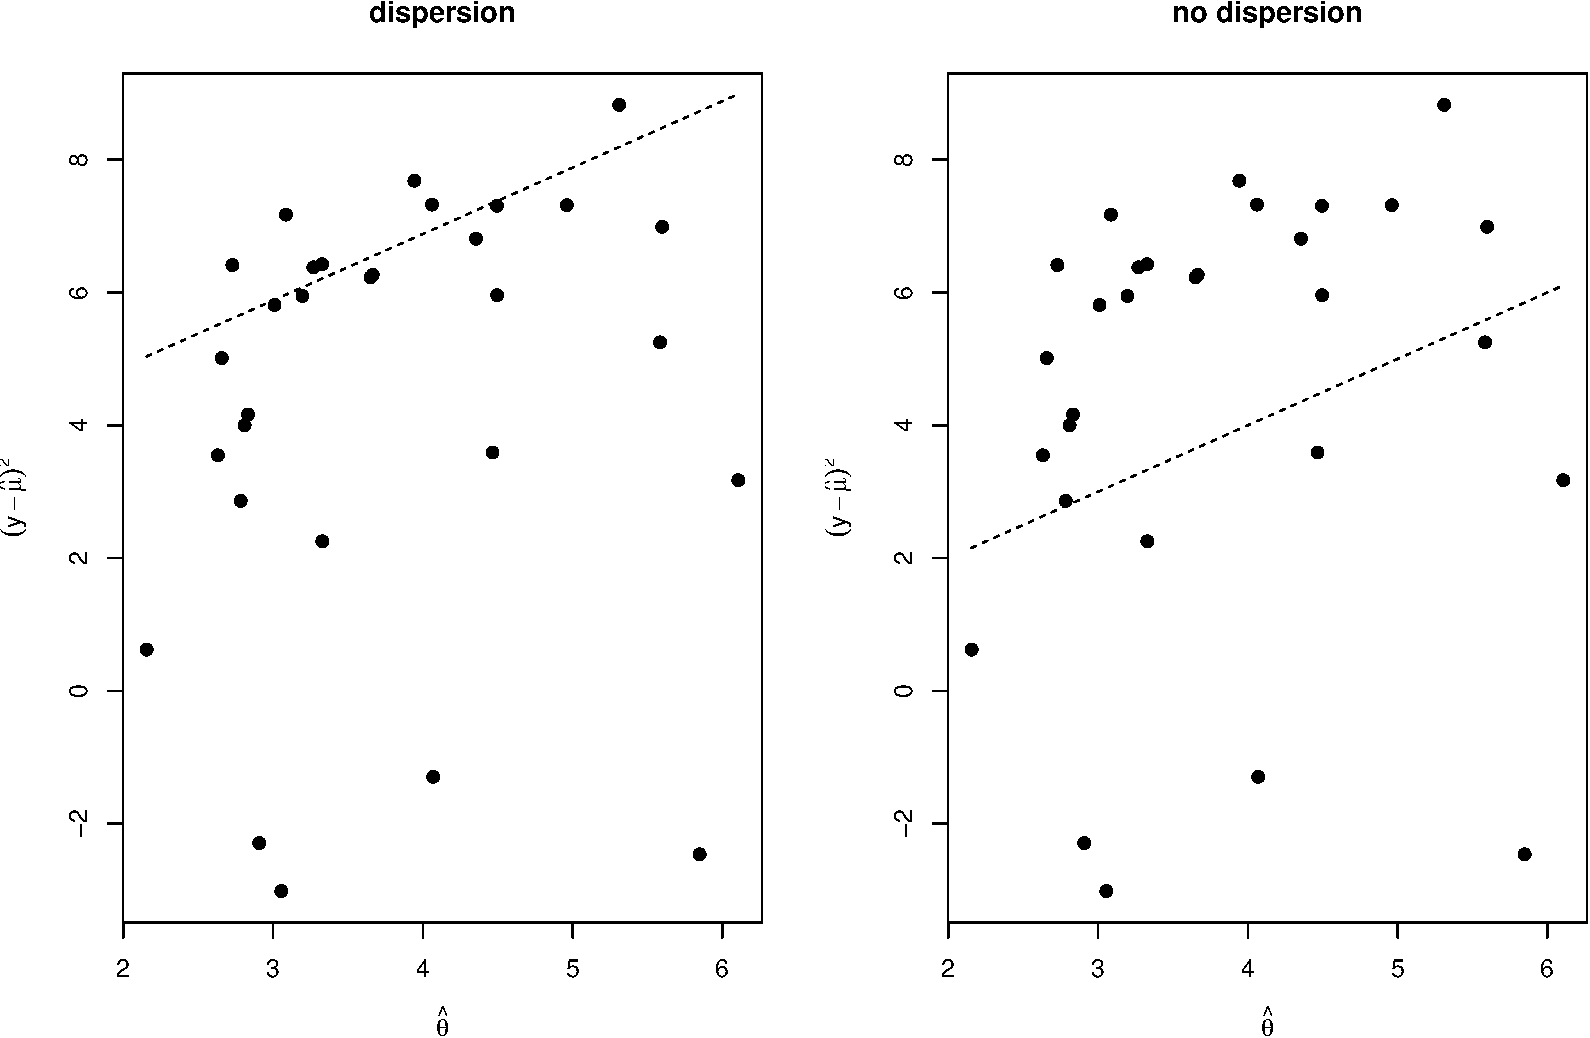
\includegraphics{week5_p1_files/figure-beamer/unnamed-chunk-12-1.pdf}
\end{frame}

\begin{frame}[fragile]{Look at residuals}
\protect\hypertarget{look-at-residuals}{}
We will now remove Santa Maria.

\vspace{12pt}
\tiny

\begin{Shaded}
\begin{Highlighting}[]
\FunctionTok{sort}\NormalTok{(}\FunctionTok{round}\NormalTok{((gala}\SpecialCharTok{$}\NormalTok{Species }\SpecialCharTok{{-}} \FunctionTok{fitted}\NormalTok{(m3))}\SpecialCharTok{\^{}}\DecValTok{2}\NormalTok{, }\DecValTok{2}\NormalTok{), }
     \AttributeTok{decreasing =} \ConstantTok{TRUE}\NormalTok{)}
\end{Highlighting}
\end{Shaded}

\begin{verbatim}
##   SantaMaria     Gardner2     Espanola        Pinta     Marchena     Gardner1 
##      6807.27      2172.44      1516.23      1504.33      1487.96      1304.18 
##  SanSalvador       Pinzon     Caldwell     Genovesa      Enderby      SantaFe 
##      1084.19       907.83       618.86       609.66       589.81       525.89 
##      Tortuga       Rabida      Seymour      Coamano SanCristobal       Onslow 
##       507.92       387.17       382.86       334.32       190.45       150.49 
##     Champion Daphne.Minor   Fernandina         Eden    SantaCruz   Las.Plazas 
##        64.28        54.63        36.26        34.75        23.89        17.49 
##    Bartolome       Darwin       Baltra Daphne.Major      Isabela         Wolf 
##         9.52         1.86         0.27         0.10         0.09         0.05
\end{verbatim}
\end{frame}

\begin{frame}[fragile]{}
\protect\hypertarget{section-14}{}
\tiny

\begin{Shaded}
\begin{Highlighting}[]
\NormalTok{m4 }\OtherTok{\textless{}{-}} \FunctionTok{glm}\NormalTok{(Species }\SpecialCharTok{\textasciitilde{}}\NormalTok{ Elevation }\SpecialCharTok{+} \FunctionTok{I}\NormalTok{(Elevation}\SpecialCharTok{\^{}}\DecValTok{2}\NormalTok{) }\SpecialCharTok{+}\NormalTok{ Nearest }\SpecialCharTok{+}\NormalTok{ Scruz }\SpecialCharTok{+} 
            \FunctionTok{I}\NormalTok{(Scruz}\SpecialCharTok{\^{}}\DecValTok{2}\NormalTok{) }\SpecialCharTok{+}\NormalTok{ Adjacent }\SpecialCharTok{+}\NormalTok{ Area }\SpecialCharTok{+} \FunctionTok{I}\NormalTok{(Area}\SpecialCharTok{\^{}}\DecValTok{2}\NormalTok{), }\AttributeTok{family =} \StringTok{"poisson"}\NormalTok{,}
            \AttributeTok{data =}\NormalTok{ gala[}\SpecialCharTok{{-}}\DecValTok{27}\NormalTok{, ], }\AttributeTok{x =} \ConstantTok{TRUE}\NormalTok{)}
\FunctionTok{summary}\NormalTok{(m4)}
\end{Highlighting}
\end{Shaded}

\begin{verbatim}
## 
## Call:
## glm(formula = Species ~ Elevation + I(Elevation^2) + Nearest + 
##     Scruz + I(Scruz^2) + Adjacent + Area + I(Area^2), family = "poisson", 
##     data = gala[-27, ], x = TRUE)
## 
## Deviance Residuals: 
##     Min       1Q   Median       3Q      Max  
## -7.4154  -2.4285  -0.0320   0.9377   6.7205  
## 
## Coefficients:
##                  Estimate Std. Error z value Pr(>|z|)    
## (Intercept)     2.442e+00  1.042e-01  23.436  < 2e-16 ***
## Elevation       5.697e-03  4.611e-04  12.355  < 2e-16 ***
## I(Elevation^2) -4.090e-06  4.650e-07  -8.796  < 2e-16 ***
## Nearest        -4.035e-03  2.475e-03  -1.630 0.103063    
## Scruz           6.016e-03  1.685e-03   3.570 0.000357 ***
## I(Scruz^2)     -2.944e-05  5.956e-06  -4.943 7.70e-07 ***
## Adjacent        2.368e-04  8.877e-05   2.667 0.007648 ** 
## Area            2.160e-03  1.785e-04  12.103  < 2e-16 ***
## I(Area^2)      -2.191e-07  3.251e-08  -6.740 1.58e-11 ***
## ---
## Signif. codes:  0 '***' 0.001 '**' 0.01 '*' 0.05 '.' 0.1 ' ' 1
## 
## (Dispersion parameter for poisson family taken to be 1)
## 
##     Null deviance: 3205.62  on 28  degrees of freedom
## Residual deviance:  356.08  on 20  degrees of freedom
## AIC: 527.42
## 
## Number of Fisher Scoring iterations: 5
\end{verbatim}
\end{frame}

\begin{frame}[fragile]{}
\protect\hypertarget{section-15}{}
Let's calculate dispersion for this new model

\vspace{12pt}
\tiny

\begin{Shaded}
\begin{Highlighting}[]
\NormalTok{p }\OtherTok{\textless{}{-}} \FunctionTok{length}\NormalTok{(}\FunctionTok{coef}\NormalTok{(m4))}
\NormalTok{n }\OtherTok{\textless{}{-}} \FunctionTok{nrow}\NormalTok{(gala) }\SpecialCharTok{{-}} \DecValTok{1}
\NormalTok{y }\OtherTok{\textless{}{-}}\NormalTok{ gala[}\SpecialCharTok{{-}}\DecValTok{27}\NormalTok{, ]}\SpecialCharTok{$}\NormalTok{Species}

\DocumentationTok{\#\# estimate dispersion directly}
\NormalTok{fits }\OtherTok{\textless{}{-}} \FunctionTok{predict}\NormalTok{(m4, }\AttributeTok{type =} \StringTok{"response"}\NormalTok{)}
\NormalTok{dp4 }\OtherTok{\textless{}{-}} \FunctionTok{sum}\NormalTok{((y }\SpecialCharTok{{-}}\NormalTok{ fits)}\SpecialCharTok{\^{}}\DecValTok{2}\SpecialCharTok{/}\NormalTok{fits) }\SpecialCharTok{/}\NormalTok{ (n }\SpecialCharTok{{-}}\NormalTok{ p)}
\NormalTok{dp4}
\end{Highlighting}
\end{Shaded}

\begin{verbatim}
## [1] 16.39359
\end{verbatim}

\begin{Shaded}
\begin{Highlighting}[]
\FunctionTok{dispersiontest}\NormalTok{(m4, }\AttributeTok{trafo=}\DecValTok{1}\NormalTok{)}
\end{Highlighting}
\end{Shaded}

\begin{verbatim}
## 
##  Overdispersion test
## 
## data:  m4
## z = 3.3744, p-value = 0.0003698
## alternative hypothesis: true alpha is greater than 0
## sample estimates:
##    alpha 
## 10.31668
\end{verbatim}
\end{frame}

\begin{frame}{}
\protect\hypertarget{section-16}{}
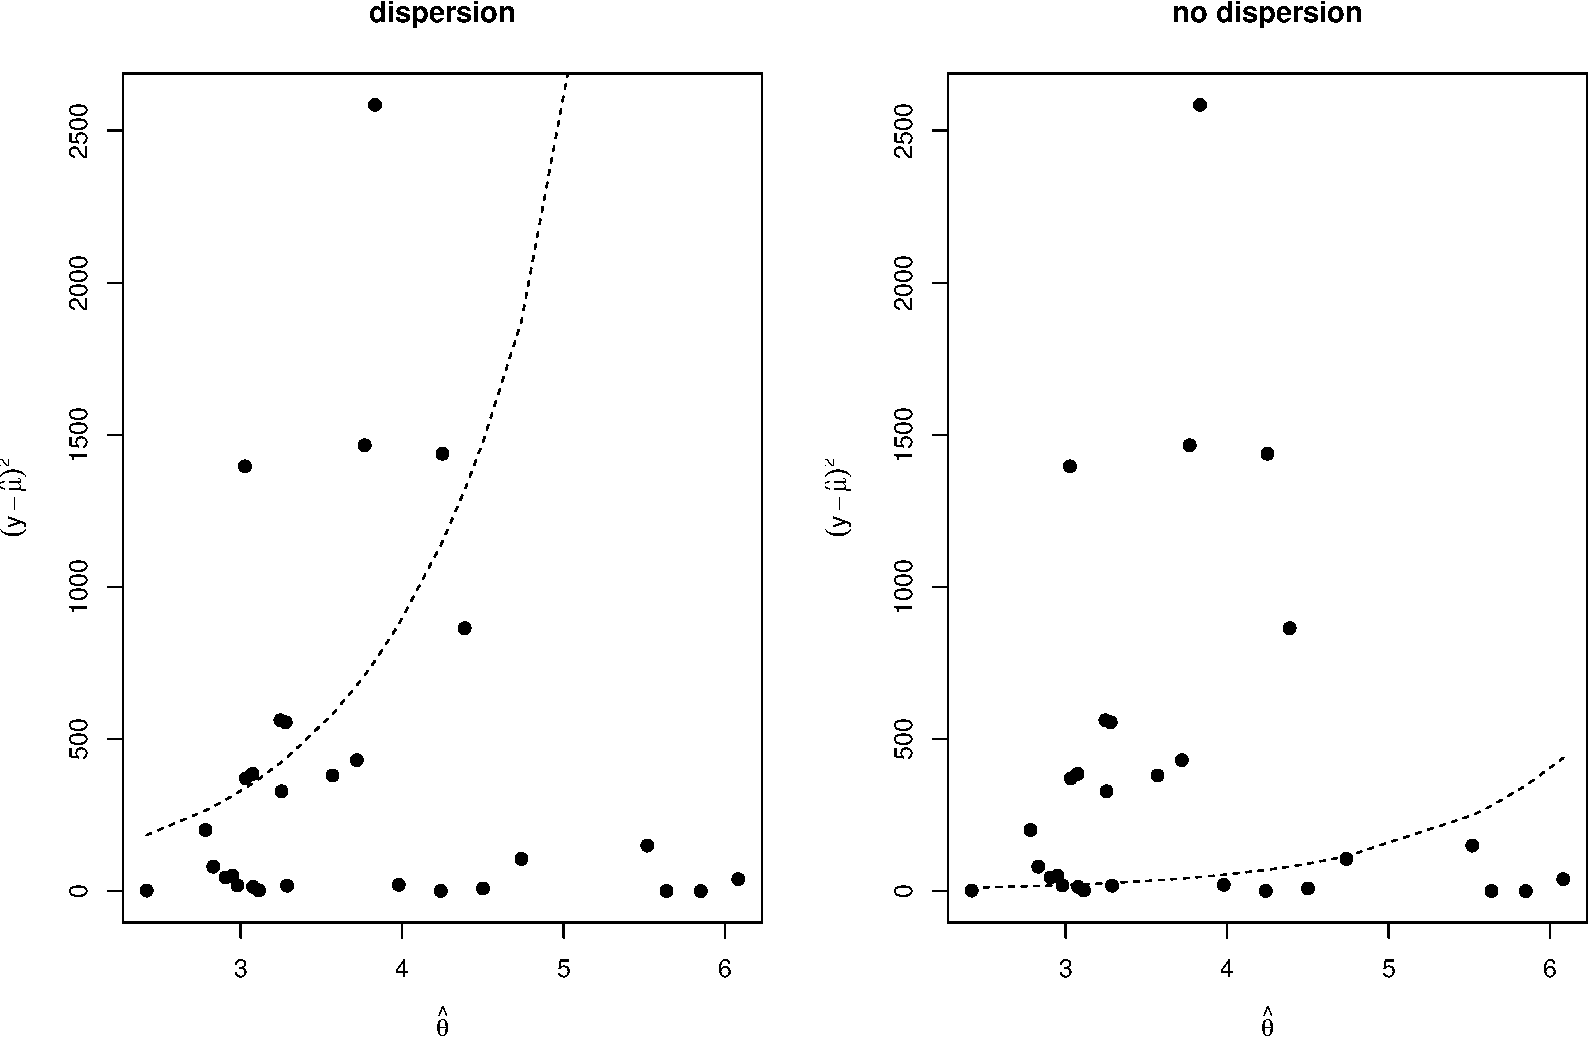
\includegraphics{week5_p1_files/figure-beamer/unnamed-chunk-16-1.pdf}
\end{frame}

\begin{frame}{}
\protect\hypertarget{section-17}{}
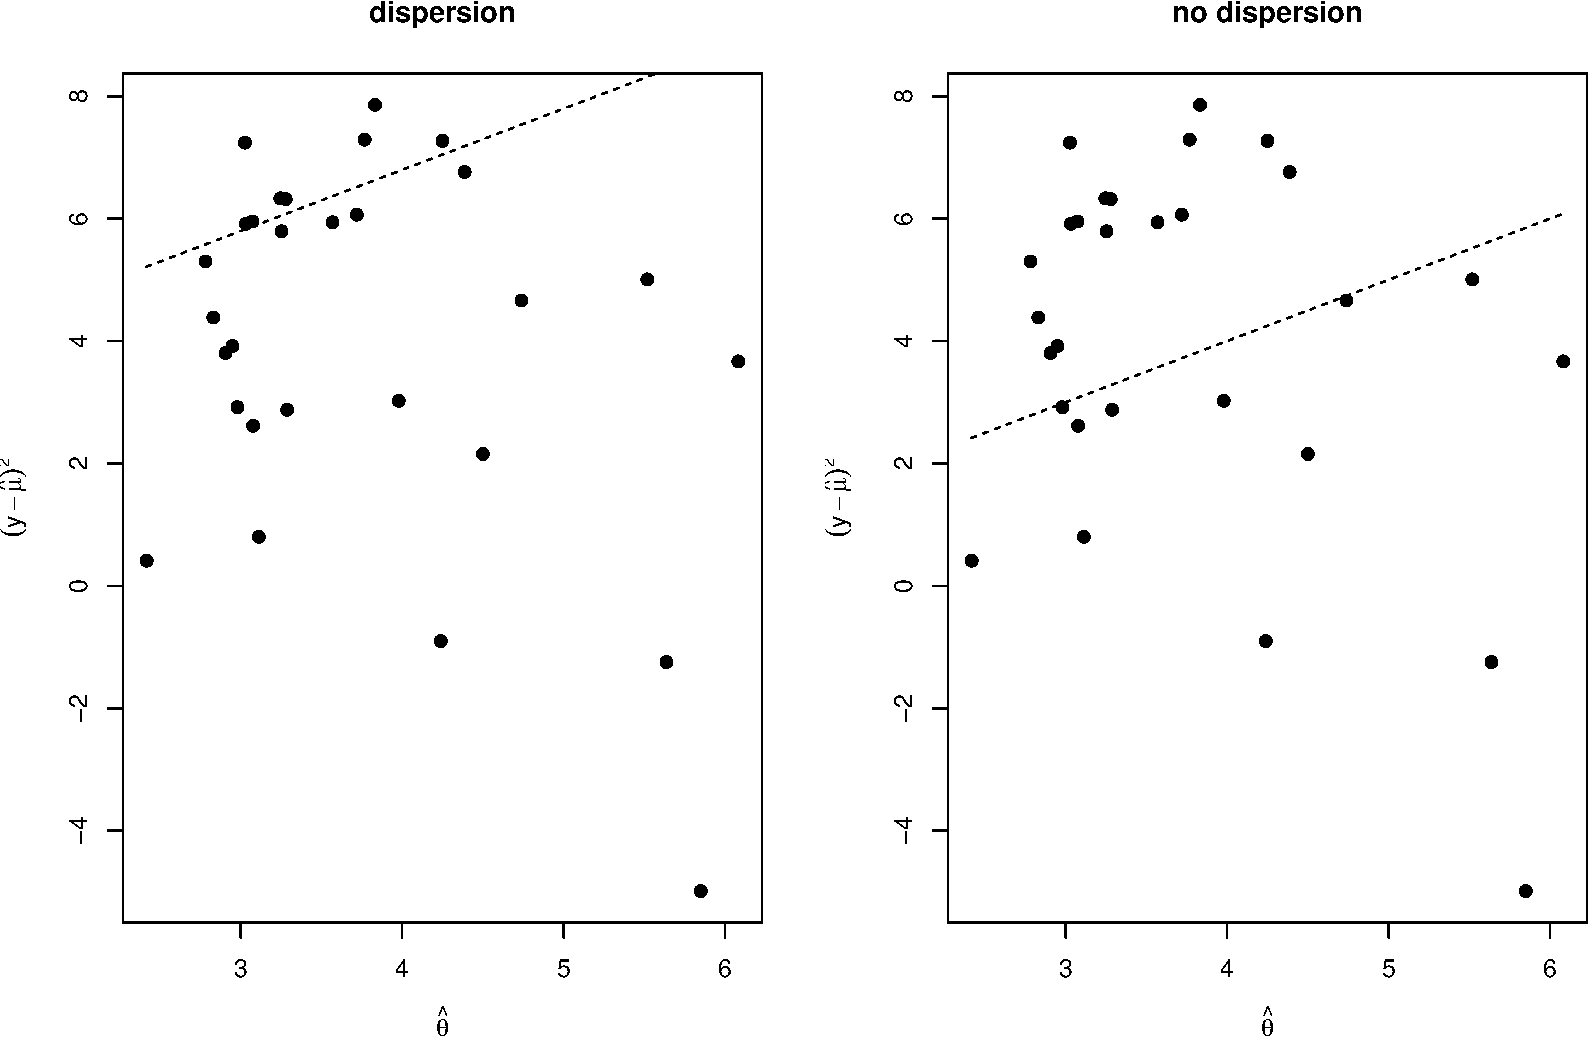
\includegraphics{week5_p1_files/figure-beamer/unnamed-chunk-17-1.pdf}
\end{frame}

\begin{frame}[fragile]{}
\protect\hypertarget{section-18}{}
Matching of large species counts is pretty good.

\vspace{12pt}
\tiny

\begin{Shaded}
\begin{Highlighting}[]
\NormalTok{foo }\OtherTok{\textless{}{-}} \FunctionTok{data.frame}\NormalTok{(}\AttributeTok{names =} \FunctionTok{rownames}\NormalTok{(gala[}\SpecialCharTok{{-}}\DecValTok{27}\NormalTok{, ]),}
                  \AttributeTok{Species =}\NormalTok{ y,}
                  \AttributeTok{pred =} \FunctionTok{as.numeric}\NormalTok{(}\FunctionTok{predict}\NormalTok{(m4, }\AttributeTok{type =} \StringTok{"response"}\NormalTok{)), }
                  \AttributeTok{resid =} \FunctionTok{residuals}\NormalTok{(m4))}
\FunctionTok{head}\NormalTok{(}\FunctionTok{cbind}\NormalTok{(foo }\SpecialCharTok{\%\textgreater{}\%} \FunctionTok{arrange}\NormalTok{(}\FunctionTok{desc}\NormalTok{(Species)) }\SpecialCharTok{\%\textgreater{}\%} \FunctionTok{pull}\NormalTok{(names),}
\NormalTok{           foo }\SpecialCharTok{\%\textgreater{}\%} \FunctionTok{arrange}\NormalTok{(}\FunctionTok{desc}\NormalTok{(pred)) }\SpecialCharTok{\%\textgreater{}\%} \FunctionTok{pull}\NormalTok{(names)), }\DecValTok{10}\NormalTok{)}
\end{Highlighting}
\end{Shaded}

\begin{verbatim}
##       [,1]           [,2]          
##  [1,] "SantaCruz"    "SantaCruz"   
##  [2,] "Isabela"      "Isabela"     
##  [3,] "SanCristobal" "SanCristobal"
##  [4,] "SanSalvador"  "SanSalvador" 
##  [5,] "Pinzon"       "Pinta"       
##  [6,] "Pinta"        "Fernandina"  
##  [7,] "Espanola"     "Marchena"    
##  [8,] "Fernandina"   "Pinzon"      
##  [9,] "Rabida"       "Rabida"      
## [10,] "SantaFe"      "Baltra"
\end{verbatim}
\end{frame}

\begin{frame}[fragile]{}
\protect\hypertarget{section-19}{}
There are still some misses, mostly among small counts.

\vspace{12pt}
\tiny

\begin{Shaded}
\begin{Highlighting}[]
\NormalTok{foo }\SpecialCharTok{\%\textgreater{}\%} \FunctionTok{arrange}\NormalTok{(}\FunctionTok{desc}\NormalTok{(}\FunctionTok{abs}\NormalTok{(resid))) }\SpecialCharTok{\%\textgreater{}\%} \FunctionTok{head}\NormalTok{(}\DecValTok{10}\NormalTok{)}
\end{Highlighting}
\end{Shaded}

\begin{verbatim}
##             names Species     pred     resid
## Gardner2 Gardner2       5 43.28636 -7.415439
## Gardner1 Gardner1      58 20.63096  6.720517
## Espanola Espanola      97 46.15761  6.510695
## Enderby   Enderby       2 25.69789 -6.097764
## Caldwell Caldwell       3 26.55618 -5.833392
## Coamano   Coamano       2 21.62974 -5.453054
## Onslow     Onslow       2 16.16162 -4.468251
## Pinzon     Pinzon     108 70.08212  4.192417
## Genovesa Genovesa      40 20.74950  3.742670
## Tortuga   Tortuga      16 35.49805 -3.673642
\end{verbatim}
\end{frame}

\begin{frame}[fragile]{Which model?}
\protect\hypertarget{which-model}{}
We can additionally consider information criteria:

\vspace{12pt}
\tiny

\begin{Shaded}
\begin{Highlighting}[]
\FunctionTok{AIC}\NormalTok{(m1, m3, m4)}
\end{Highlighting}
\end{Shaded}

\begin{verbatim}
## Warning in AIC.default(m1, m3, m4): models are not all fitted to the same number
## of observations
\end{verbatim}

\begin{verbatim}
##    df      AIC
## m1  7 769.0063
## m3  9 590.7201
## m4  9 527.4177
\end{verbatim}

\begin{Shaded}
\begin{Highlighting}[]
\FunctionTok{BIC}\NormalTok{(m1, m3, m4)}
\end{Highlighting}
\end{Shaded}

\begin{verbatim}
## Warning in BIC.default(m1, m3, m4): models are not all fitted to the same number
## of observations
\end{verbatim}

\begin{verbatim}
##    df      BIC
## m1  7 778.8146
## m3  9 603.3309
## m4  9 539.7234
\end{verbatim}
\end{frame}

\begin{frame}{Negative Binomial regression}
\protect\hypertarget{negative-binomial-regression}{}
Given a series of independent trials, each trial with probability of
success \(p\), let \(Z\) be the number of trials until the \(k\)th
success.

\vspace{12pt}

The negative binomial distribution can arise naturally in a few ways:

\begin{itemize}
\tightlist
\item
  One can envision a system that can withstand \(k\) hits before
  failure. The probability of a hit in a given time period is \(p\).
\item
  The negative binomial also arises from the generalization of the
  Poisson where the rate parameter is gamma distributed.
\end{itemize}
\end{frame}

\begin{frame}{}
\protect\hypertarget{section-20}{}
The mass function for the negative binomial distribution is: \[
  \mathbb{P}(Z = z) = {z-1 \choose k-1}p^k(1-p)^{z-k}, \qquad z = k,k+1,\ldots,
\]

\vspace{12pt}

We get a more convenient parameterization if we let \(Y = Z - k\) and
\(p = (1 + \alpha)^{-1}\) so that: \[
  \mathbb{P}(Y=y) = {y+k-1 \choose k-1} \frac{\alpha^y}{(1+\alpha)^{y+k}}, \qquad y = 0,1,2,\ldots.
\] Then \(\mathrm{E}(Y) = \mu = k\alpha\) and
\(\mathrm{Var}(Y) = k\alpha + k\alpha^2 = \mu + \mu^2/k\). The
log-likelihood is then \[
  \sum_{i=1}^n\left(y_i\log\left(\frac{\alpha}{1 + \alpha}\right) - k\log(1 + \alpha) 
    + \sum_{j=0}^{y_i-1}\log(j+k) - \log(y_i!)\right).
\]
\end{frame}

\begin{frame}{}
\protect\hypertarget{section-21}{}
\begin{center}
Can the log likelihood on the previous slide be written in canonical form?
\end{center}
\end{frame}

\begin{frame}{}
\protect\hypertarget{section-22}{}
The most convenient way to link the mean response \(\mu\) to a linear
combination of the the predictors \(X\) in typical GLM fashion is
through \[
  \log\left(\frac{\mu}{\mu+k}\right) = \log\left(\frac{\alpha}{1+\alpha}\right) = \theta = x'\beta.
\]

\vspace{12pt}

We can specify the change of parameters map \(g:\theta\to\mu\) and the
link function as \(g^{-1}:\mu\to\theta\) as \[
  g(\theta) = \frac{ke^\theta}{1 - e^\theta} = \mu, \qquad 
    g^{-1}(\mu) = \log\left(\frac{\mu}{\mu+k}\right) = x'\beta.
\]

\vspace{12pt}

We can regard \(k\) as fixed and determined by the application or as an
additional parameter to be estimated.
\end{frame}

\begin{frame}{Example: Solder data}
\protect\hypertarget{example-solder-data}{}
ATT ran an experiment varying five factors relevant to a wave-soldering
procedure for mounting components on printed circuit boards.

\vspace{12pt}

The response variable, skips, is a count of how many solder skips
appeared in a visual inspection.

\vspace{12pt}

The data comes from Comizzoli et al.~(1990) (See the source material on
the help page for the solder dataset in the faraway package).
\end{frame}

\begin{frame}[fragile]{}
\protect\hypertarget{section-23}{}
We start with a Poisson regression:

\vspace{12pt}
\tiny

\begin{Shaded}
\begin{Highlighting}[]
\FunctionTok{library}\NormalTok{(faraway)}
\NormalTok{modp }\OtherTok{\textless{}{-}} \FunctionTok{glm}\NormalTok{(skips }\SpecialCharTok{\textasciitilde{}}\NormalTok{ . , }\AttributeTok{family=}\NormalTok{poisson, }\AttributeTok{data=}\NormalTok{solder)}
\FunctionTok{c}\NormalTok{(}\FunctionTok{deviance}\NormalTok{(modp), }\FunctionTok{df.residual}\NormalTok{(modp))}
\end{Highlighting}
\end{Shaded}

\begin{verbatim}
## [1] 1796.973  881.000
\end{verbatim}

We see that the full model has a residual deviance of 1797 on 881
degrees of freedom. This is not a good fit (as a rule of thumb, deviance
should be less than degrees of freedom for a well-fitting submodel).
\end{frame}

\begin{frame}[fragile]{}
\protect\hypertarget{section-24}{}
Perhaps including interaction terms will improve the fit:

\vspace{12pt}
\tiny

\begin{Shaded}
\begin{Highlighting}[]
\NormalTok{modp2 }\OtherTok{\textless{}{-}} \FunctionTok{glm}\NormalTok{(skips }\SpecialCharTok{\textasciitilde{}}\NormalTok{ (Opening }\SpecialCharTok{+}\NormalTok{Solder }\SpecialCharTok{+}\NormalTok{ Mask }\SpecialCharTok{+}\NormalTok{ PadType }\SpecialCharTok{+}\NormalTok{ Panel)}\SpecialCharTok{\^{}}\DecValTok{2}\NormalTok{, }
             \AttributeTok{family=}\NormalTok{poisson, }\AttributeTok{data=}\NormalTok{solder)}
\FunctionTok{c}\NormalTok{(}\FunctionTok{deviance}\NormalTok{(modp2), }\FunctionTok{df.residual}\NormalTok{(modp2))}
\end{Highlighting}
\end{Shaded}

\begin{verbatim}
## [1] 1007.736  773.000
\end{verbatim}

\begin{Shaded}
\begin{Highlighting}[]
\FunctionTok{pchisq}\NormalTok{(}\FunctionTok{deviance}\NormalTok{(modp2), }\FunctionTok{df.residual}\NormalTok{(modp2), }\AttributeTok{lower=}\ConstantTok{FALSE}\NormalTok{)}
\end{Highlighting}
\end{Shaded}

\begin{verbatim}
## [1] 2.238499e-08
\end{verbatim}

\vspace{12pt}
\normalsize

The fit is improved but not enough to conclude that the model fits. We
could investigate:

\begin{itemize}
\tightlist
\item
  adding more interactions but that would make interpretation
  increasingly difficult.
\item
  A check for outliers reveals no problem.
\end{itemize}
\end{frame}

\begin{frame}{Try negative binomial regression}
\protect\hypertarget{try-negative-binomial-regression}{}
The functions for fitting come from the \texttt{MASS} package. Note that
the \texttt{MASS} package has a \texttt{select} function that will clash
with the \texttt{select} function in \texttt{dplyr}. Write
\texttt{dplyr::select} for data wrangling.

\vspace{12pt}

We can specify the link parameter \(k\). Here we choose \(k = 1\) to
demonstrate the method, although there is no substantive motivation from
this application to use this value.

\vspace{12pt}

Note that the \(k = 1\) case corresponds to an assumption of a geometric
distribution for the response.
\end{frame}

\begin{frame}[fragile]{}
\protect\hypertarget{section-25}{}
\tiny

\begin{Shaded}
\begin{Highlighting}[]
\FunctionTok{library}\NormalTok{(MASS)}
\end{Highlighting}
\end{Shaded}

\begin{verbatim}
## 
## Attaching package: 'MASS'
\end{verbatim}

\begin{verbatim}
## The following object is masked from 'package:dplyr':
## 
##     select
\end{verbatim}

\begin{Shaded}
\begin{Highlighting}[]
\NormalTok{modn }\OtherTok{\textless{}{-}} \FunctionTok{glm}\NormalTok{(skips }\SpecialCharTok{\textasciitilde{}}\NormalTok{ ., }\FunctionTok{negative.binomial}\NormalTok{(}\DecValTok{1}\NormalTok{), solder)}
\NormalTok{modn}
\end{Highlighting}
\end{Shaded}

\begin{verbatim}
## 
## Call:  glm(formula = skips ~ ., family = negative.binomial(1), data = solder)
## 
## Coefficients:
## (Intercept)     OpeningM     OpeningS   SolderThin       MaskA3       MaskA6  
##    -1.57251      0.50852      2.00093      1.04754      0.65065      2.52776  
##      MaskB3       MaskB6    PadTypeD6    PadTypeD7    PadTypeL4    PadTypeL6  
##     1.26631      2.07062     -0.45434      0.01979      0.46751     -0.46812  
##   PadTypeL7    PadTypeL8    PadTypeL9    PadTypeW4    PadTypeW9       Panel2  
##    -0.28999     -0.08057     -0.51864     -0.13917     -1.48133      0.29536  
##      Panel3  
##     0.34262  
## 
## Degrees of Freedom: 899 Total (i.e. Null);  881 Residual
## Null Deviance:       1743 
## Residual Deviance: 556.7     AIC: 3884
\end{verbatim}

\begin{Shaded}
\begin{Highlighting}[]
\DocumentationTok{\#\# LRT test}
\FunctionTok{pchisq}\NormalTok{(}\FunctionTok{deviance}\NormalTok{(modn), }\FunctionTok{df.residual}\NormalTok{(modn), }\AttributeTok{lower=}\ConstantTok{FALSE}\NormalTok{)}
\end{Highlighting}
\end{Shaded}

\begin{verbatim}
## [1] 1
\end{verbatim}
\end{frame}

\begin{frame}[fragile]{}
\protect\hypertarget{section-26}{}
We can estimate the parameter \(k\) using maximum likelihood estimation
in:

\tiny

\begin{Shaded}
\begin{Highlighting}[]
\NormalTok{modn }\OtherTok{\textless{}{-}} \FunctionTok{glm.nb}\NormalTok{(skips }\SpecialCharTok{\textasciitilde{}}\NormalTok{ ., solder)}
\FunctionTok{summary}\NormalTok{(modn)}
\end{Highlighting}
\end{Shaded}

\begin{verbatim}
## 
## Call:
## glm.nb(formula = skips ~ ., data = solder, init.theta = 4.52811339, 
##     link = log)
## 
## Deviance Residuals: 
##     Min       1Q   Median       3Q      Max  
## -2.7047  -1.0109  -0.3921   0.4480   2.8869  
## 
## Coefficients:
##             Estimate Std. Error z value Pr(>|z|)    
## (Intercept) -1.29859    0.13202  -9.837  < 2e-16 ***
## OpeningM     0.50353    0.07932   6.348 2.18e-10 ***
## OpeningS     1.91104    0.07111  26.876  < 2e-16 ***
## SolderThin   0.93513    0.05323  17.567  < 2e-16 ***
## MaskA3       0.58383    0.09592   6.087 1.15e-09 ***
## MaskA6       2.26096    0.10101  22.384  < 2e-16 ***
## MaskB3       1.20651    0.09572  12.605  < 2e-16 ***
## MaskB6       1.98172    0.09158  21.638  < 2e-16 ***
## PadTypeD6   -0.46189    0.11145  -4.144 3.41e-05 ***
## PadTypeD7   -0.03182    0.10584  -0.301 0.763655    
## PadTypeL4    0.38119    0.10177   3.745 0.000180 ***
## PadTypeL6   -0.57860    0.11327  -5.108 3.25e-07 ***
## PadTypeL7   -0.36569    0.11006  -3.323 0.000891 ***
## PadTypeL8   -0.15882    0.10734  -1.480 0.138953    
## PadTypeL9   -0.56554    0.11306  -5.002 5.67e-07 ***
## PadTypeW4   -0.19851    0.10783  -1.841 0.065630 .  
## PadTypeW9   -1.56332    0.13538 -11.547  < 2e-16 ***
## Panel2       0.29574    0.06322   4.678 2.90e-06 ***
## Panel3       0.33380    0.06298   5.300 1.16e-07 ***
## ---
## Signif. codes:  0 '***' 0.001 '**' 0.01 '*' 0.05 '.' 0.1 ' ' 1
## 
## (Dispersion parameter for Negative Binomial(4.5281) family taken to be 1)
## 
##     Null deviance: 4097.6  on 899  degrees of freedom
## Residual deviance: 1012.1  on 881  degrees of freedom
## AIC: 3679.5
## 
## Number of Fisher Scoring iterations: 1
## 
## 
##               Theta:  4.528 
##           Std. Err.:  0.518 
## 
##  2 x log-likelihood:  -3639.514
\end{verbatim}
\end{frame}

\begin{frame}[fragile]{}
\protect\hypertarget{section-27}{}
We see that \(\hat k = 4.528\) with a standard error of \(0.518\).

\vspace{12pt}

We can compare negative binomial models using the usual inferential
techniques. For instance, we see that the overall fit is much improved.

\vspace{12pt}
\tiny

\begin{Shaded}
\begin{Highlighting}[]
\DocumentationTok{\#\# LRT test}
\FunctionTok{pchisq}\NormalTok{(}\FunctionTok{deviance}\NormalTok{(modn), }\FunctionTok{df.residual}\NormalTok{(modn), }\AttributeTok{lower=}\ConstantTok{FALSE}\NormalTok{)}
\end{Highlighting}
\end{Shaded}

\begin{verbatim}
## [1] 0.001367546
\end{verbatim}
\end{frame}

\begin{frame}{Zero Inflated Count Models}
\protect\hypertarget{zero-inflated-count-models}{}
Sometimes we see count response data where the number of zeroes
appearing is significantly greater than the Poisson or negative binomial
models would predict.

\vspace{12pt}

This commonly arises in

\begin{itemize}
\tightlist
\item
  life history analyses of plants and animals where many subjects die
  before they reproduce, arrest
\item
  bookings data where many people are either not arrested or receive
  zero day sentences,
\item
  insurance claims data.
\end{itemize}

\vspace{12pt}

Modifying the Poisson by adding a dispersion parameter does not
adequately model this divergence from the standard count distributions.
\end{frame}

\begin{frame}{Biochemistry graduate students}
\protect\hypertarget{biochemistry-graduate-students}{}
We consider a sample of 915 biochemistry graduate students.

\vspace{12pt}

The response variable is the number of articles produced during the last
three years of the PhD. \vspace{12pt} We are interested in how this is
influenced by the gender, marital status, number of children, prestige
of the department and productivity of the advisor of the student.

\vspace{12pt}

The dataset may be found in the \texttt{pscl} package.
\end{frame}

\begin{frame}[fragile]{}
\protect\hypertarget{section-28}{}
We start by fitting a Poisson regression model:

\vspace{12pt}
\tiny

\begin{Shaded}
\begin{Highlighting}[]
\FunctionTok{library}\NormalTok{(pscl)}
\NormalTok{modp }\OtherTok{\textless{}{-}} \FunctionTok{glm}\NormalTok{(art }\SpecialCharTok{\textasciitilde{}}\NormalTok{ ., }\AttributeTok{data=}\NormalTok{bioChemists, }\AttributeTok{family=}\NormalTok{poisson)}
\FunctionTok{sumary}\NormalTok{(modp)}
\end{Highlighting}
\end{Shaded}

\begin{verbatim}
##               Estimate Std. Error z value  Pr(>|z|)
## (Intercept)  0.3046168  0.1029814  2.9580  0.003097
## femWomen    -0.2245942  0.0546135 -4.1124 3.915e-05
## marMarried   0.1552434  0.0613744  2.5294  0.011424
## kid5        -0.1848827  0.0401269 -4.6075 4.076e-06
## phd          0.0128226  0.0263970  0.4858  0.627139
## ment         0.0255427  0.0020061 12.7327 < 2.2e-16
## 
## n = 915 p = 6
## Deviance = 1634.37098 Null Deviance = 1817.40530 (Difference = 183.03432)
\end{verbatim}
\end{frame}

\begin{frame}{}
\protect\hypertarget{section-29}{}
We can see that deviance is significantly larger than the degrees of
freedom (a rule of thumb indicated poor fit).

\vspace{12pt}

Some experimentation reveals that this cannot be solved by using a
richer linear predictor or by eliminating some outliers (see Faraway).

\vspace{12pt}

We might consider a dispersed Poisson model or negative binomial but
some thought suggests that there are good reasons why a disproportionate
number of students might produce no articles at all.
\end{frame}

\begin{frame}[fragile]{}
\protect\hypertarget{section-30}{}
We count and predict how many students produce between zero and seven
articles. Very few students produce more than seven articles so we
ignore these.

\vspace{12pt}

The \texttt{predprob} function produces the predicted probabilities for
each case. By summing these, we get the expected number for each article
count.

\vspace{12pt}
\tiny

\begin{Shaded}
\begin{Highlighting}[]
\NormalTok{ocount }\OtherTok{\textless{}{-}} \FunctionTok{table}\NormalTok{(bioChemists}\SpecialCharTok{$}\NormalTok{art)[}\DecValTok{1}\SpecialCharTok{:}\DecValTok{8}\NormalTok{]}
\NormalTok{pcount }\OtherTok{\textless{}{-}} \FunctionTok{colSums}\NormalTok{(}\FunctionTok{predprob}\NormalTok{(modp)[,}\DecValTok{1}\SpecialCharTok{:}\DecValTok{8}\NormalTok{])}
\end{Highlighting}
\end{Shaded}
\end{frame}

\begin{frame}[fragile]{}
\protect\hypertarget{section-31}{}
\tiny

\begin{Shaded}
\begin{Highlighting}[]
\FunctionTok{plot}\NormalTok{(pcount, ocount, }\AttributeTok{type=}\StringTok{"n"}\NormalTok{, }\AttributeTok{xlab=}\StringTok{"Predicted"}\NormalTok{, }\AttributeTok{ylab=}\StringTok{"Observed"}\NormalTok{, }
     \AttributeTok{ylim =} \FunctionTok{c}\NormalTok{(}\DecValTok{0}\NormalTok{, }\DecValTok{300}\NormalTok{), }\AttributeTok{axes =} \ConstantTok{FALSE}\NormalTok{)}
\FunctionTok{axis}\NormalTok{(}\AttributeTok{side =} \DecValTok{1}\NormalTok{)}
\FunctionTok{axis}\NormalTok{(}\AttributeTok{side =} \DecValTok{2}\NormalTok{)}
\FunctionTok{text}\NormalTok{(pcount,ocount, }\DecValTok{0}\SpecialCharTok{:}\DecValTok{7}\NormalTok{)}
\end{Highlighting}
\end{Shaded}

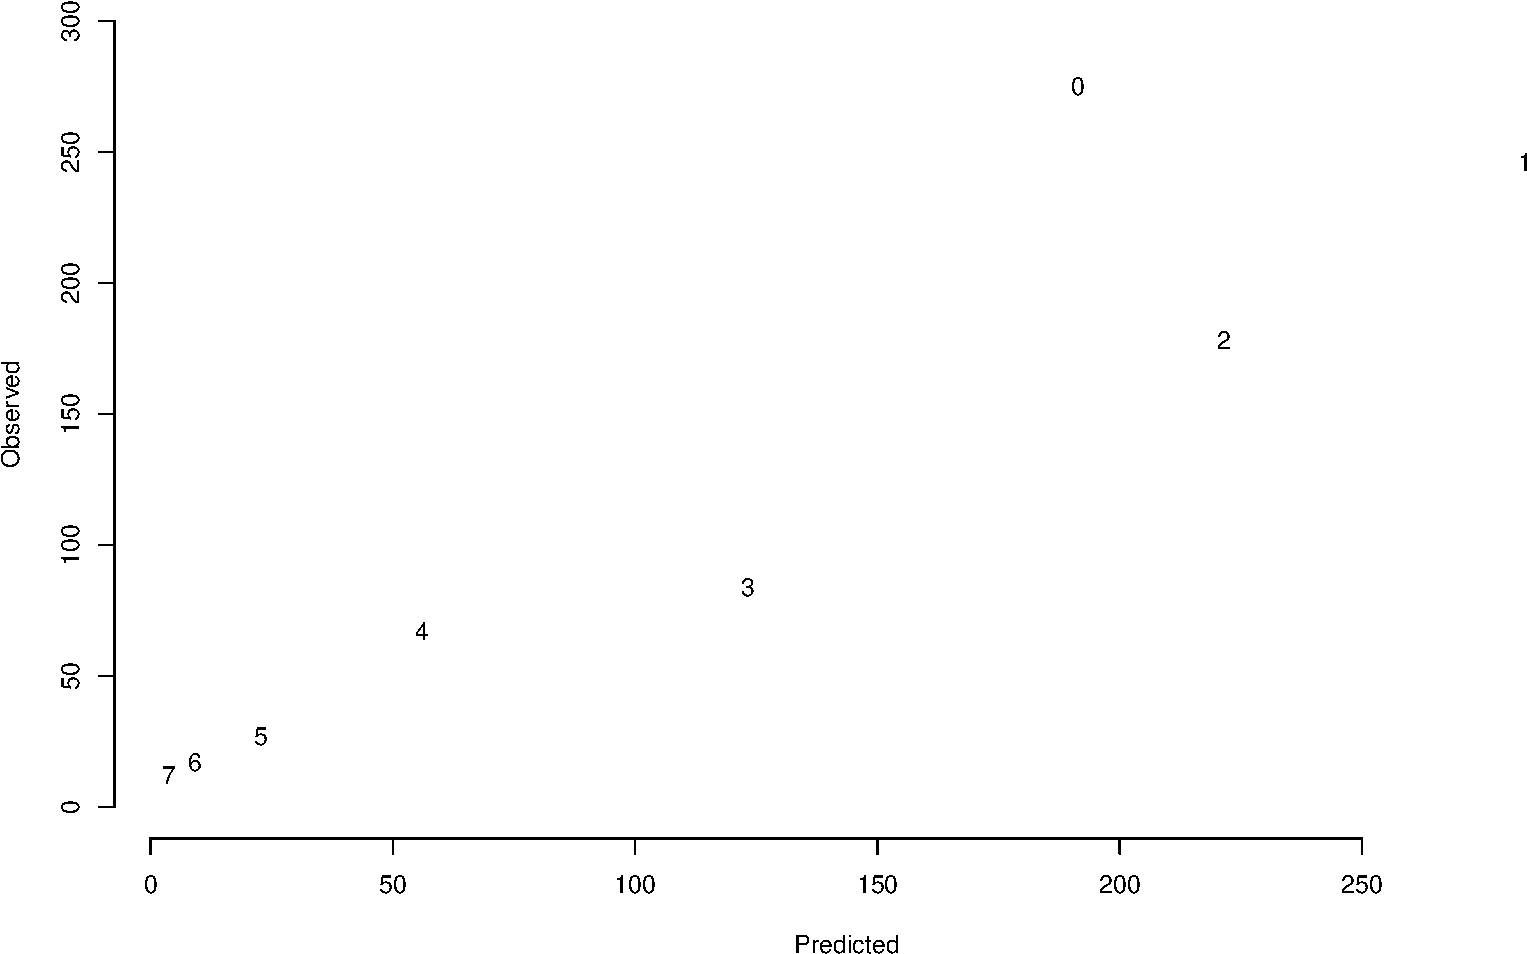
\includegraphics{week5_p1_files/figure-beamer/unnamed-chunk-28-1.pdf}
\end{frame}

\end{document}
